\documentclass[12pt, letter, oneside]{book}
\usepackage{fancyhdr, ifpdf}
\usepackage{float}
\usepackage{setspace}
\usepackage{color}
\usepackage{xcolor}
\usepackage{listings}
\usepackage{caption}
\usepackage[ampersand]{easylist}
\usepackage{amssymb}
\usepackage{pdflscape}
\usepackage{verbatim}
\usepackage{longtable}
\usepackage[margin=1cm]{caption}
\usepackage[top=1in, bottom=.75in, left=.7in, right=1in]{geometry}
\ListProperties(Hide=100, Hang=true, Progressive=3ex,Style*=$\bullet$ , Style2*=-- )

\definecolor{mygray}{rgb}{0.9,0.9,0.9}
\lstdefinestyle{customc}{
  backgroundcolor=\color{mygray},
  captionpos=b, 
  belowcaptionskip=1\baselineskip,
  breaklines=true,
  numbers=left,
  numberstyle=\footnotesize,
  %frame=L,
  xleftmargin=\parindent,
  language=C++,
  showstringspaces=false,
  basicstyle=\footnotesize\ttfamily,
  keywordstyle=\bfseries\color{green!40!black},
  commentstyle=\itshape\color{purple!40!black},
  identifierstyle=\color{black},
  stringstyle=\color{cyan}  
}

\lstset{escapechar=@,style=customc,tabsize=4}

%% some redefination of the headers and footers
\renewcommand{\chaptermark}[1]%
                 {\markboth{#1}{}}
\renewcommand{\sectionmark}[1]%
                 {\markright{\thesection\ #1}}
\lhead[\fancyplain{}{\thepage}]%
      {\fancyplain{}{\rightmark}}
\rhead[\fancyplain{}{\leftmark}]%
      {\fancyplain{}{\thepage}}
\cfoot{}
\sloppy

\ifpdf
   \usepackage[pdftex]{graphicx}
   \usepackage{rotating}
\else
   \usepackage{graphicx}
	\usepackage{rotating}   
\fi

\graphicspath{{./Figures/}}
\doublespacing

\begin{document}
\doublespace

\clearpage
\pagenumbering{arabic}

\setcounter{chapter}{0}

\chapter{Parameter Minimization using the Levenberg-Marquardt algorithm}
\emph{Do some fitting}
\section{Introduction}
The Levenberg-Marquardt plugin is used to fit a proposed SBML models parameters to experimental data. 

The current implementation is based on the lmfit C library by Joachim Wuttke. See footnote\footnote{The package lmfit is distributed under the FreeBSD License:

--
  Copyright (c) 2013 Joachim Wuttke All rights reserved.

  Redistribution and use in source and binary forms, with or without
  modification, are permitted provided that the following conditions are met:

  - Redistributions of source code must retain the above copyright notice,
    this list of conditions and the following disclaimer.
  - Redistributions in binary form must reproduce the above copyright notice,
    this list of conditions and the following disclaimer in the documentation
    and/or other materials provided with the distribution.

  This software is provided by the copyright holders and contributors "as is"
  and any express or implied warranties, including, but not limited to, the
  implied warranties of merchantability and fitness for a particular purpose
  are disclaimed. In no event shall the copyright holder or contributors
  be liable for any direct, indirect, incidental, special, exemplary, or
  consequential damages (including, but not limited to, procurement of
  substitute goods or services; loss of use, data, or profits; or business
  interruption) however caused and on any theory of liability, whether in
  contract, strict liability, or tort (including negligence or otherwise)
  arising in any way out of the use of this software, even if advised of the
  possibility of such damage.
--} for full license disclosure.

The current plugin has one capability, named \verb|LMFit|. The plugin has numerous parameters, as documented below.

\section{Plugin Parameters}
In the following, plugin parameters available in the Levenberg-Marquardt plugin are discussed.

\begin{table}[ht]
\centering % used for centering table
\begin{tabular}{l l p{7.5cm}} % centered columns (4 columns)

Parameter Name & Data Type & Purpose \\ [0.5ex] % inserts table 
%heading
\hline % inserts single horizontal line
ObservedData   				& 	RoadRunnerData 		& 	Input data.  \\
ModelData      				& 	RoadRunnerData    	& 	Output data. \\
ResidualsData  				& 	RoadRunnerData    	& 	Residuals data (difference between input and output data.) \\
InputParameterList 			&	Parameters   		& 	Parameters to fit \\
OutputParameterList 		&   Parameters  	 	& 	Parameters, and their numbers, that were fitted \\
ObservedDataSelectionList 	& 	StringList			&	Species selection list for observed data \\
ModelDataSelectionList 		& 	StringList			&	Selection list for model data \\
Norm						&	double				& 	Norm of fitting. An estimate of goodness of fit. \\

\hline %inserts single line
\end{tabular}
\caption{LM fit plugin parameters} 
\label{table:lmfitPluginParameters} 
\end{table}

\section{Plugin Callbacks}
\begin{table}[ht]
\centering % used for centering table
\begin{tabular}{l l p{7.5cm}} % centered columns (4 columns)

Callback & Arguments & Purpose \\ [0.5ex] % inserts table 
%heading
\hline % inserts single horizontal line
PluginStarted  	& 	void*, & Signal to application that the plugin has started. \\
PluginProgress	& 	int*  & Signal progress of fitting, in \% (0-100\%). \\
PluginFinished	& 	void* & Signal to application the plugin has finished. \\

\hline %inserts single line
\end{tabular}
\caption{LMFit Plugin callbacks} 
\label{table:lmfitPluginCallBacks} 
\end{table}

\section{The \texttt{execute()} function}
The lmfit plugins \verb|execute()| function supports two arguments;

\verb|execute(void* rrData, bool workInThread)|

where \verb|rrData| is a handle to RoadRunner data and \verb|workInThread| is a boolean denoting if the work is to be executed in a thread or not.

\section{Python example}

\begin{singlespace}
\lstinputlisting[label=plugin_lmfit_header,caption={Minimization example.},language=Python]{Examples/lmfitPlugin/rrLevenbergMarquardtDemo.py}
\end{singlespace}

\begin{figure}[H]
\centering
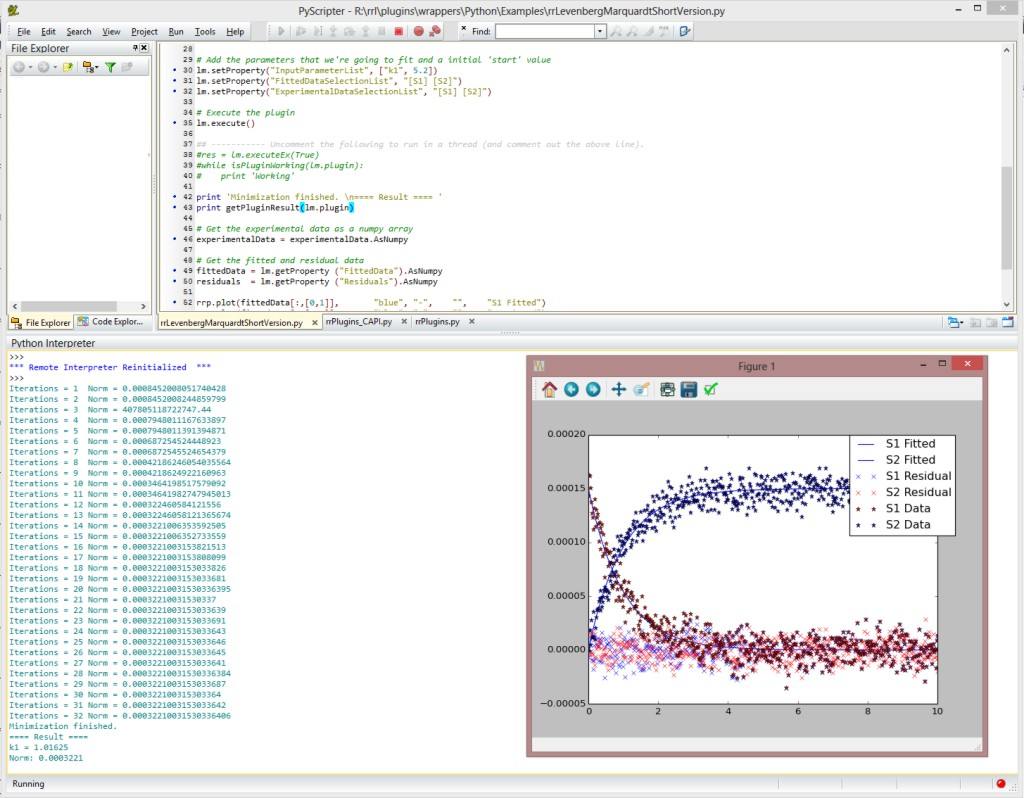
\includegraphics[width=120mm]{Minimization.jpg}
\caption{Output fot the LMFit python example script discussed above}
\label{fig:lmfitFig}
\end{figure}






\end{document}






